\chapter{Results and Discussion}
\label{Chap:Results}

\section{Introduction to Results and Discussion}
In this chapter we will present our results for this project and discuss their significance and shortcomings.\todo{finish this}

\section{Local Air Temperature and SIC Correlations}
\begin{figure}[H]
    \centering
    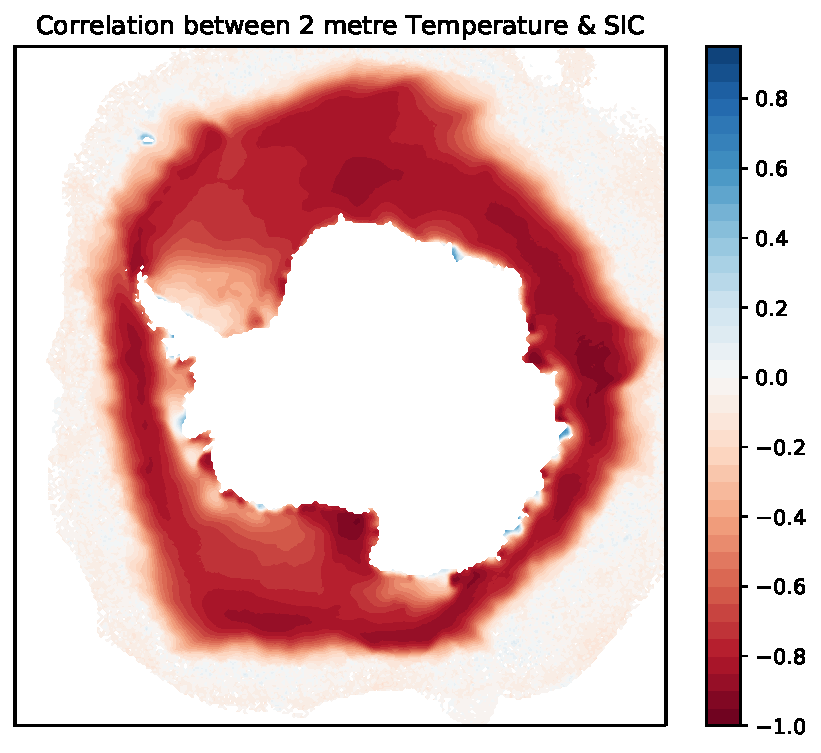
\includegraphics{Images/tempcorrwithsic.pdf}
    \caption{Correlation between temperature at 2m with sea ice concentration.}
    \label{fig:results:2mtemp_corr_with_sic}
\end{figure}
Above we have the correlation between 2 metre air temperature and sea ice concentration over Antarctica. The result that the temperature is negatively correlated with the concentration of sea ice in Antarctica is hardly surprising. Higher temperatures will be associated in the melting of ice. This both intuitively makes sense and is supported by the first law of thermodynamics (Conservation of energy). The main feature of interest in this plot is the regions which are close to the pole and there are lower correlations between 2m-temperature and SIC. It is possible that this is due to low variability in SIC in these regions over the entirety of each year.


\section{Global Temperature and SIC Extent}
In light of work done by other researchers which looked at global temperature correlated with the total amount of sea ice in Antarctica. \cite{Wang2019Compounding2016, Meehl2019Sustained2016} we carried out this comparison ourselves. Taking the Pearson correlation between the time series of 2m temperature at each gridpoint globally with the time series of total sea ice in Antarctica.

\begin{figure}[H]
    \centering
    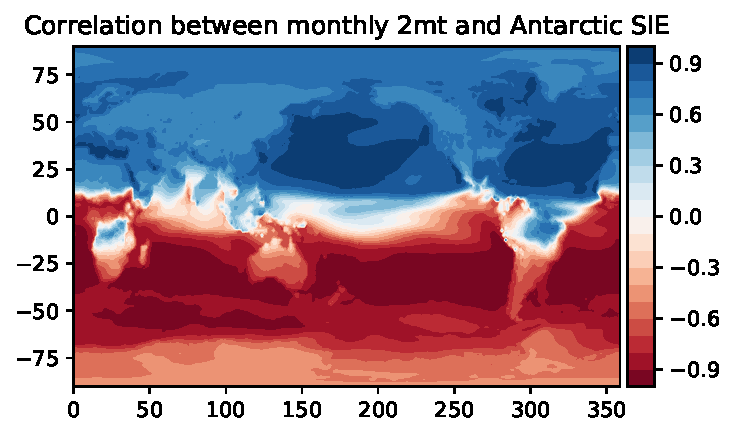
\includegraphics{Images/global_correlation_2mt_sie.pdf}
    \caption{Correlation between 2m temperature and total SIE in Antarctica.}
    \label{fig:my_label}
\end{figure}
I haven't done any preprocessing with this data so far. I believe the papers looked at some kind of anomaly in the amount of sea ice, as such I will look into doing something similar next week.
What we see here however is good as we see a positive correlation in the northern hemisphere and a negative correlation in the southern hemisphere.